%%%%%%%%%%%%%%%%%%%
%%% 2023-08-15 %%%%
%%%%%%%%%%%%%%%%%%%
\section{Encuadre (2024-08-15)}
\begin{frame}\frametitle{Presentación del curso}
  \textbf{Objetivos:}
  \begin{itemize}
  \item Aprender los conceptos básicos para operar un robot móvil autónomo
  \item Implementar dichos conceptos en un ambiente simulado
  \item Familiarizar al estudiante con la plataforma ROS
  \end{itemize}
\end{frame}

\begin{frame}\frametitle{Ubicación en el plan de estudios}
  Bloque de ingeniería aplicada:
  \begin{figure}
    \centering
    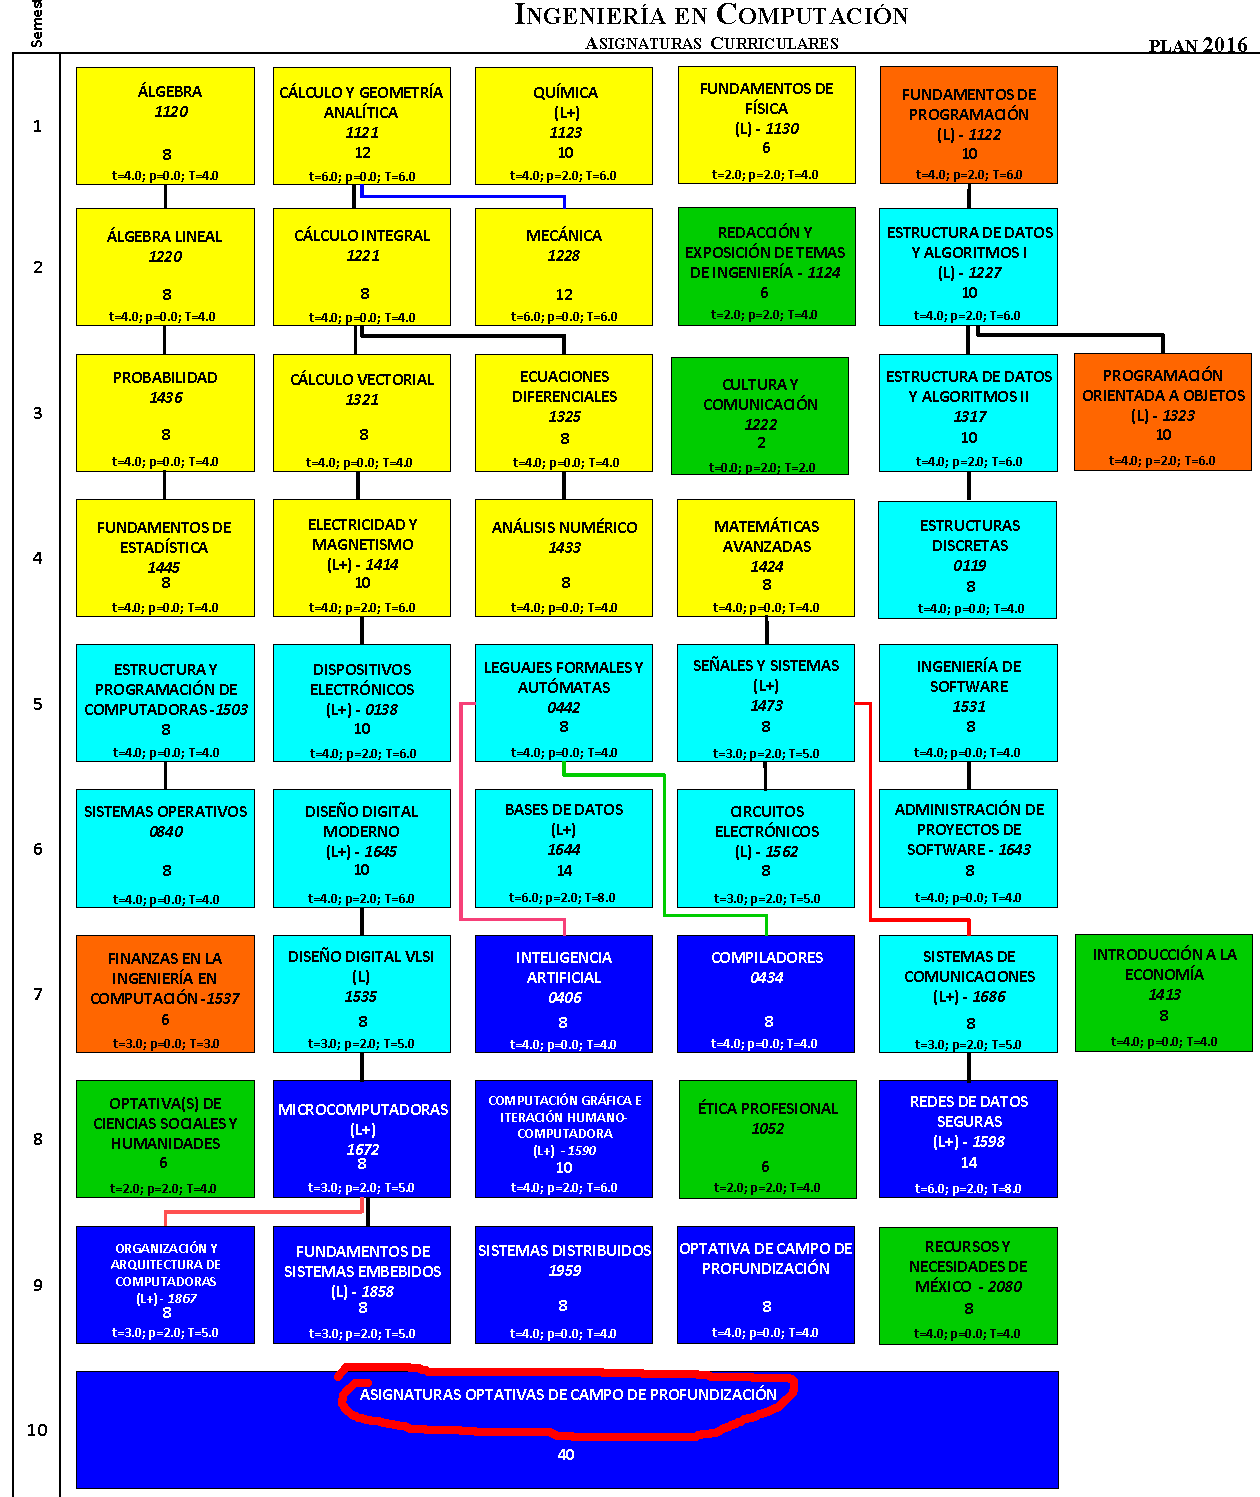
\includegraphics[width=0.3\textwidth]{Figures/PlanComputacion.png}
    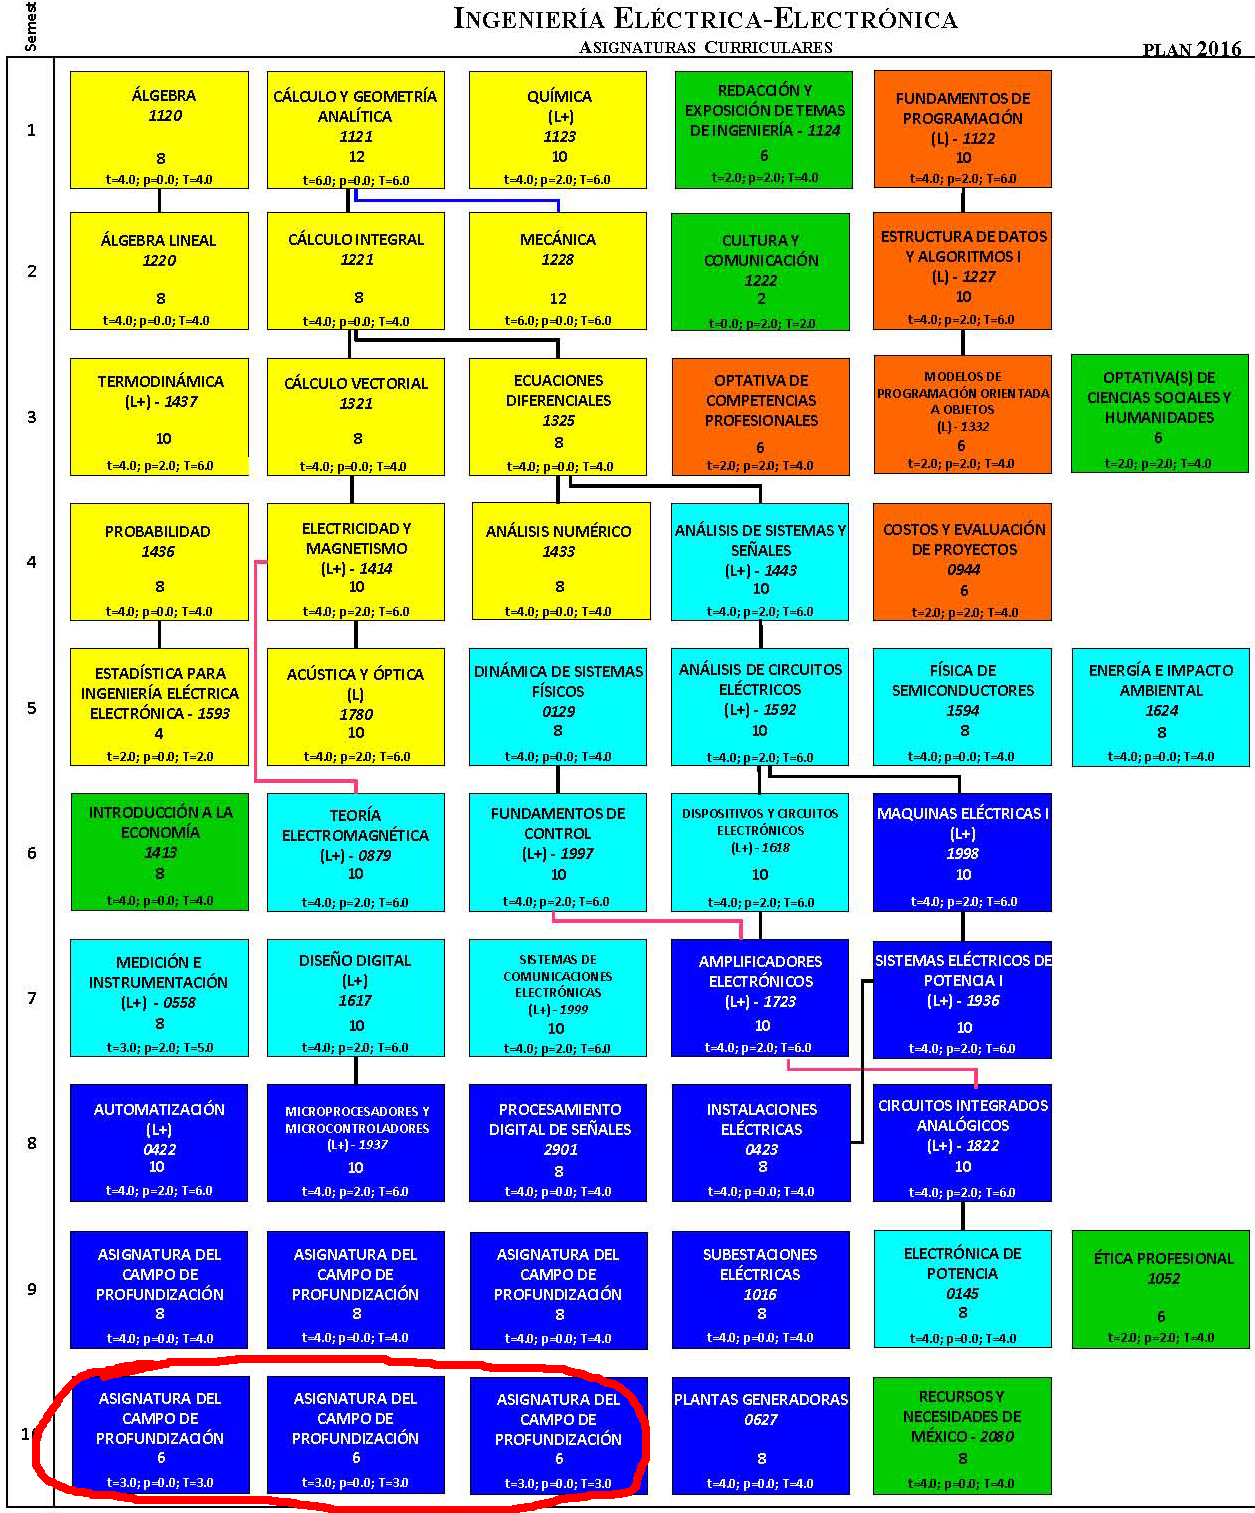
\includegraphics[width=0.3\textwidth]{Figures/PlanElectronica.png}
    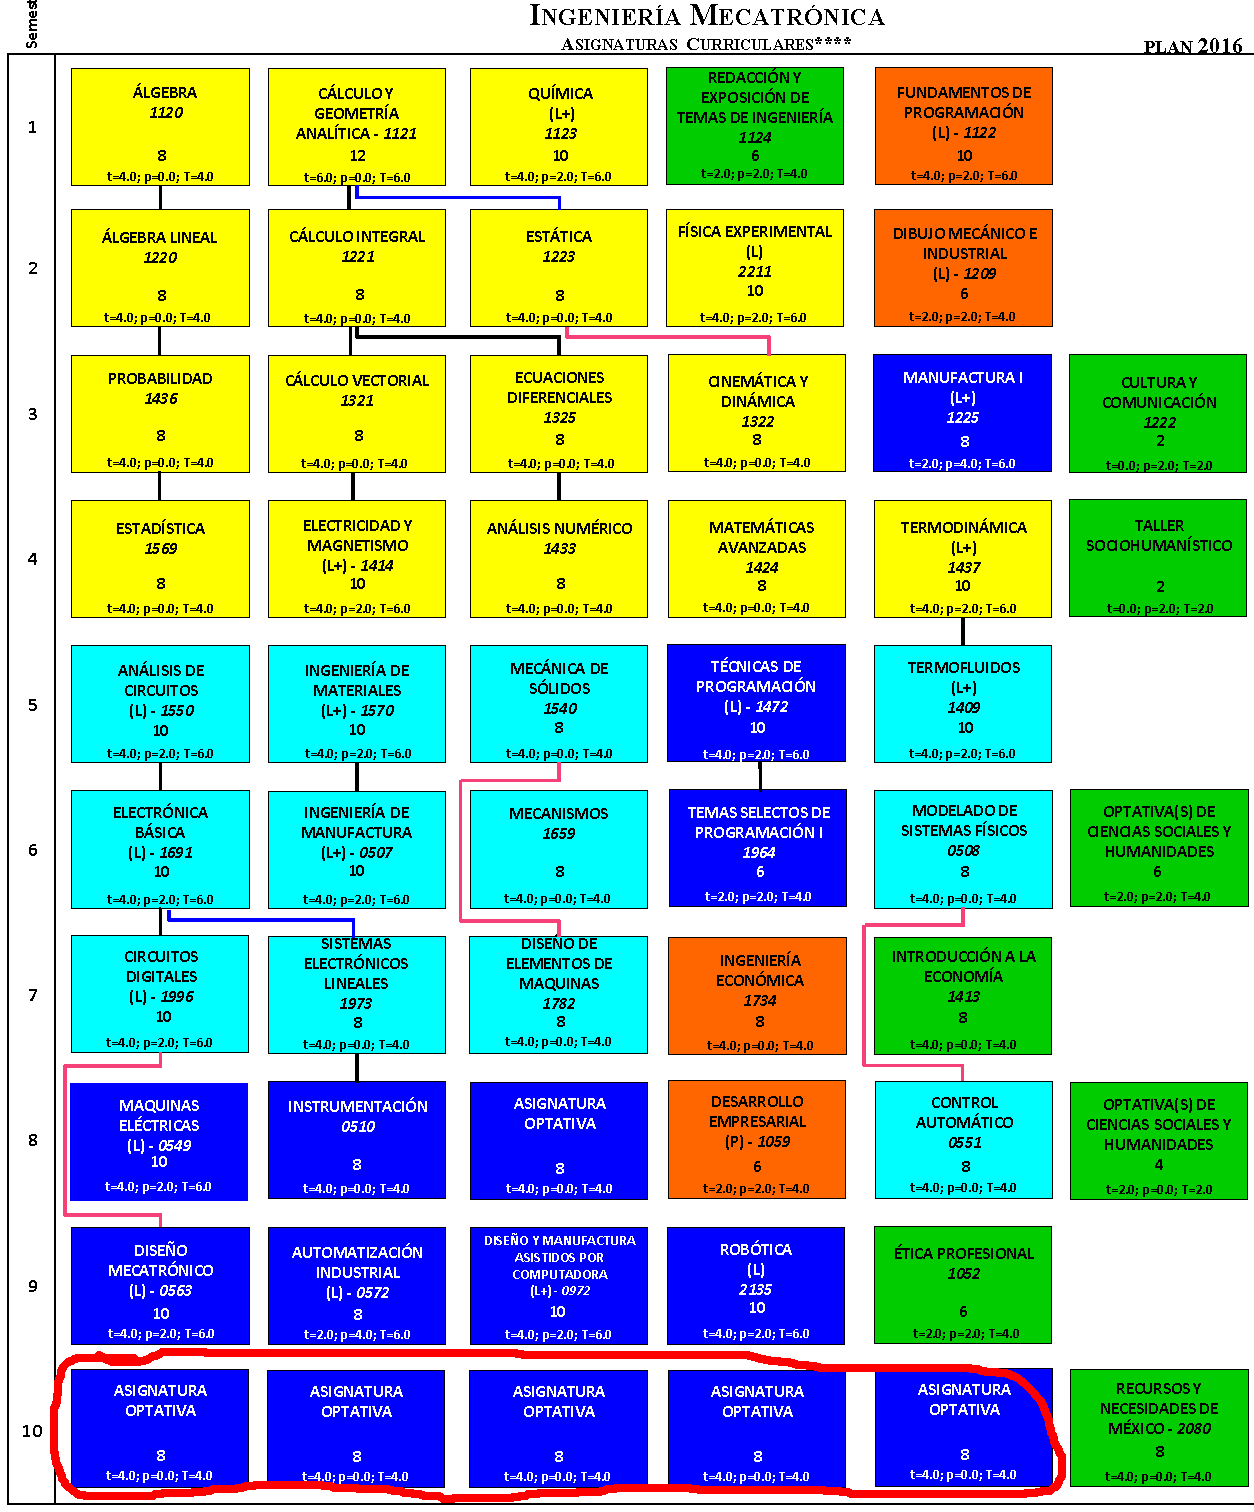
\includegraphics[width=0.3\textwidth]{Figures/PlanMecatronica.png}
  \end{figure}
  El curso integra diversos conceptos vistos a lo largo de la carrera: cálculo, álgebra, geometría, probabilidad, estructuras de datos, control, entre otras. 
\end{frame}

\begin{frame}\frametitle{Contenido}
  \begin{enumerate}
  \item Introducción y generalidades
    \begin{itemize}
    \item Componentes básicos de un robot móvil
    \item Modelos tradicionales, reactivos e híbridos
    \item Herramientas de software para el desarrollo de robots móviles
    \end{itemize}
  \item Planeación de movimientos
    \begin{itemize}
    \item El problema de la planeación de movimientos
    \item Mapas geométricos y topológicos
    \item Descomposición en celdas, celdas de ocupación y diagramas de Voronoi
    \item Planeación de rutas mediante búsqueda en grafos
    \item Modelos cinemáticos: diferencial, omnidireccional, Ackermann
    \item Control de posición y seguimiento de trayectorias
    \end{itemize}
  \item Modelos reactivos
    \begin{itemize}
    \item Máquinas de estados finitas
    \item Campos potenciales artificiales
    \item Navegación mediante redes neuronales
    \item Navegación mediante algoritmos genéticos
    \end{itemize}
  \end{enumerate}
\end{frame}

\begin{frame}\frametitle{Contenido}
  \begin{enumerate}
    \setcounter{enumi}{3}
  \item Mapeo y localización
    \begin{itemize}
    \item Localización mediante Modelos Ocultos de Markov
    \item Localización mediante filtros de partículas
    \item Creación de mapas mediante agrupamiento
    \item Localización y mapeo simultáneos
    \end{itemize}
  \item Conceptos básicos de visión artificial
    \begin{itemize}
    \item Imágenes y espacios de color
    \item Operadores morfológicos
    \item Extracción de características geométricas
    \item Visión 3D mediante imágenes RGB-D
    \end{itemize}
  \item Conceptos básicos de manipulación
    \begin{itemize}
    \item Movimiento de cuerpo rígido
    \item Cinemáticas directa e inversa
    \item Planeación y seguimiento de trayectorias
    \end{itemize}
  \end{enumerate}
\end{frame}

\begin{frame}\frametitle{Contenido}
  \begin{enumerate}
    \setcounter{enumi}{6}
  \item Representación del conocimiento
    \begin{itemize}
    \item Sistemas basados en reglas
    \item Lógica difusa
    \end{itemize}
  \item Herramientas para la interacción humano-robot
    \begin{itemize}
    \item El modelo fuente-filtro para síntesis de voz
    \item Síntesis de voz con la biblioteca Festival
    \item Reconocimiento de palabras aisladas
    \item Reconocimiento de voz con la biblioteca CMU Sphinx
    \end{itemize}
  \end{enumerate}
  \textbf{Bibliografía recomendada:}
  \begin{itemize}
    \item \url{https://drive.google.com/drive/folders/1gb7VQJG5eUkCvCginRHHGn5lez6VASBJ?usp=sharing}
    \item \url{https://drive.google.com/drive/folders/1Epl2b51xEJzCvzfugBD1i7xGdKYdJucy?usp=sharing}
  \end{itemize}
  
\end{frame}

\begin{frame}\frametitle{Forma de trabajo}
  \begin{itemize}
  \item Horario: martes y jueves de 16:00 a 17:30.\\
  \item Para la realización de ciertas tareas y prácticas se utilizará el simulador Gazebo junto con la plataforma ROS Noetic. Este software corre en el sistema operativo Ubuntu 20.04.4. Varias tareas y prácticas implicarán escribir código para lo cual se utilizará el repositorio\\
    \url{https://github.com/mnegretev/Mobile-Robots-2023-2}\\
    Si no se desea instalar el sistema operativo de forma nativa, en el repositorio hay una máquina virtual con todo el software ya instalado.
  \item Para el uso del material del curso, se recomienda manejar las siguientes herramientas:
    \begin{itemize}
    \item Sistema operativo Ubuntu
    \item Lenguajes Python y C++
    \item Software de control de versiones Git
    \end{itemize}
    Un conocimiento a nivel introductorio es suficiente.
  \item Algunas actividades serán individuales y otras en equipo.
  \item Se creará una rama del repositorio para cada estudiante donde podrá subir códigos. Para ello el estudiante debe tener cuenta en GitHub (gratuita) y se le darán permisos de escritura en el repositorio. 
  \item Las tareas que impliquen la escritura de código, se subirán al repositorio en la rama asignada para cada estudiante.
  \item Las tareas que no impliquen código se entregarán en papel al inicio de la clase.
  \end{itemize}
  Habrá un grupo en Google Classroom para todos los avisos. 
\end{frame}

\begin{frame}\frametitle{Forma de evaluar}
  Rubros a evaluar:
  \begin{table}
    \textbf{
  \begin{tabular}{lr}
    Prácticas & 40\%\\
    Examen    & 30\%\\
    Tareas    & 25\%\\
    Proyecto  & 15\%
  \end{tabular}}
  \end{table}
  El examen final se exenta con 6.0. Si un alumno con calificación aprobatoria presenta el examen final, se entiende que renuncia a su calificación y el examen final contará el 100\%.\\
  \Large{\textbf{Todo comportamiento antiético causará una calificación de 0 en el entregable correspondiente.\\Copiar y pegar texto de internet es un ejemplo de esto.}}
  \normalsize
  \[\]
\end{frame}

\begin{frame}\frametitle{Forma de evaluar}
  \begin{itemize}
  \item Las tareas se entregarán en papel al inicio de la clase en la fecha de entrega asignada.
  \item Las prácticas consistirán en la escritura de código, que se subirá al repositorio en la rama correspondiente, y en la elaboración de un reporte escrito, que también se entregará impreso al inicio de la clase en la fecha asignada. 
  \item El proyecto final consistirá en la integración de los conceptos vistos en el curso, por lo que también consistirá en la escritura de código y en un reporte escrito.
  \item Los reportes de prácticas y proyecto deberán contener al menos los siguientes puntos:
    \begin{itemize}
    \item Introducción (que incluya contexto, motivación, planteamiento del problema y objetivos)
    \item Marco teórico (donde se expliquen los conceptos utilizados en la práctica o proyecto)
    \item Desarrollo (donde se expliquen la implementación y las pruebas realizadas)
    \item Resultados (donde se reporten las diferentes pruebas de funcionamiento)
    \item Conclusiones (donde se discutan los resultados obtenidos y se plantee un trabajo futuro)
    \item Referencias
    \end{itemize}
  \item No hay extensión mínima ni máxima.
  \item No es necesario que los reportes sean extensos. Se prefiere que sean concisos.
  \item Las referencias deben ser sólo \textbf{publicaciones arbitradas} (libros, artículos de revista, memorias de congresos, entre otros). Se recomienda usar el buscador de la Dirección General de Bibliotecas de la UNAM (\url{https://www.dgb.unam.mx/})
  \item Para la evaluación de los reportes escritos se utilizará la siguiente rúbrica:
  \end{itemize}
\end{frame}

\begin{frame}\frametitle{Evaluación de reportes de prácticas y proyecto}
  \begin{figure}
    \centering
    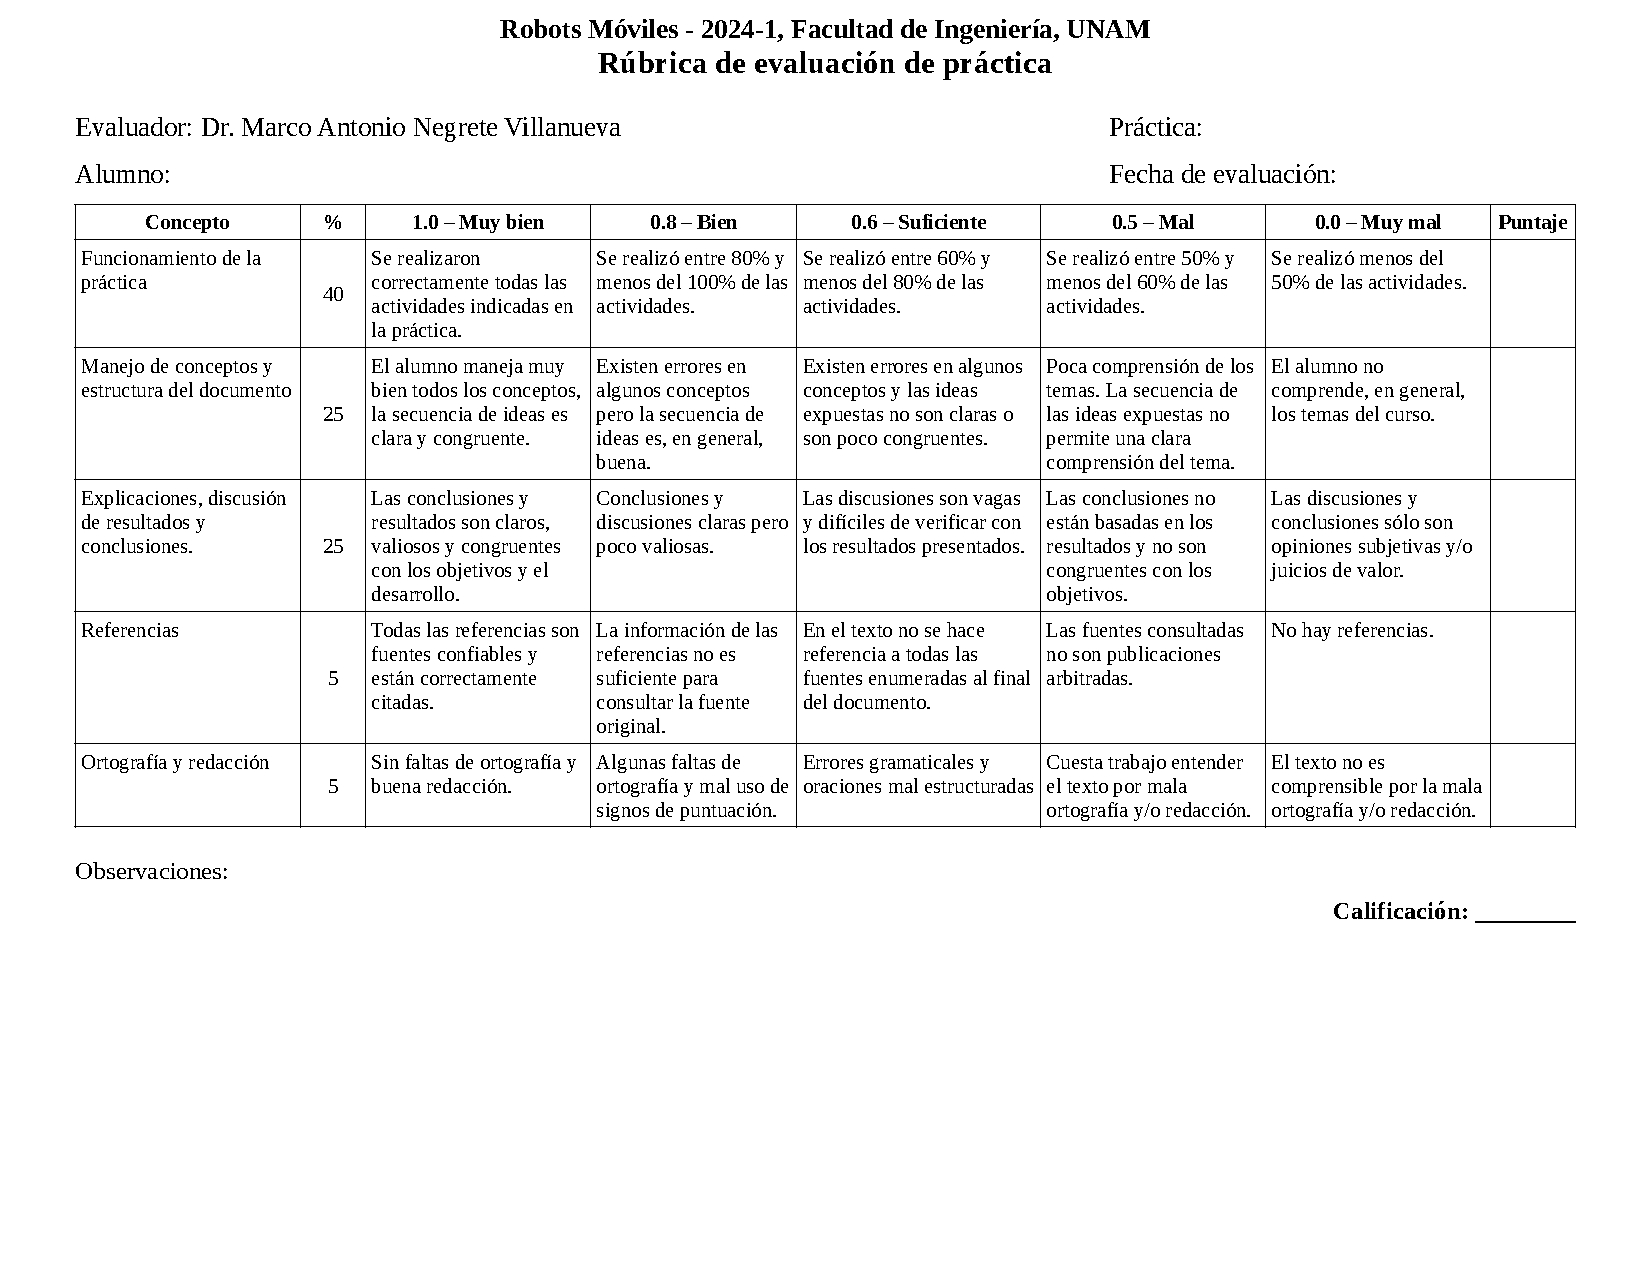
\includegraphics[height=1.25\textheight]{Figures/Rubrica.pdf}
  \end{figure}
\end{frame}

\begin{frame}\frametitle{Obligatorio}
  \textbf{Para poder continuar con el curso, todos los estudiantes deberán enviar un correo a }
  \[\]
  \texttt{marco.negrete@ingenieria.unam.edu}
  \[\]
  \textbf{indicando que están de acuerdo con la forma de evaluar.}
\end{frame}

